\chapter{vector}
\section{接口与实现}

\subsection{abstract data type}
\begin{itemize}
\item 抽象数据类型: 数据模型(抽象定义) + 一组操作
\item 数据结构: 基于特定语言(具体实现),实现ADT的一整套算法
\item 向量是数组的泛化
\begin{itemize}
\item 一组元素按照线性次序封装而成 (call by rank)
\item 各元素与rank意义对应
\item 元素类型不限于基本类型
\item 提供ADT接口操作向量
\end{itemize}
\end{itemize}

\section{可扩充向量}
\subsection{静态空间管理}
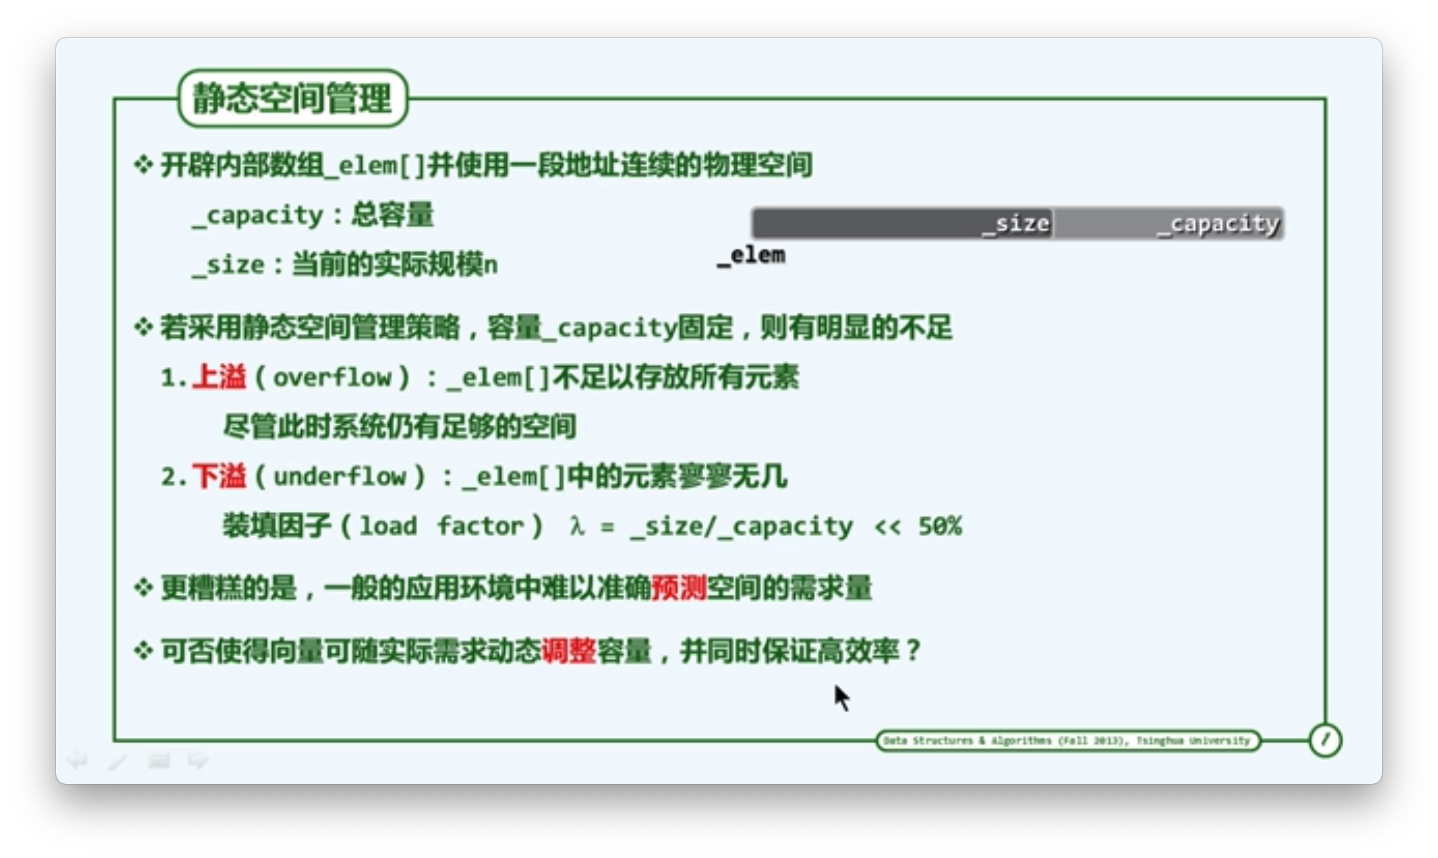
\includegraphics[scale=0.5]{3-1}

\subsection{动态空间管理}
\begin{itemize}
\item 即将发生{\color{red} 上溢}的时候,重新开辟大的内存空间,数据copy过来,原本空间释放\\
\comment{问题是以前的指针可能会出现问题}
\end{itemize}

\paragraph{递增式扩容}
每加入I个元素就需要扩容一次,在I、2I、3I... m*I个元素时扩容,扩容时间$=I^{*}(m-1) * m / 2=0\left(n^{2}\right)$, $O(n^2)$,每次扩容的分摊成本$O(n)$。

\paragraph{加倍式扩容}
在连续插入1、2、4、8... $2^m$的时候扩容,总体耗时$=O(n)$,每次扩容的分摊成本是$O(1)$\\
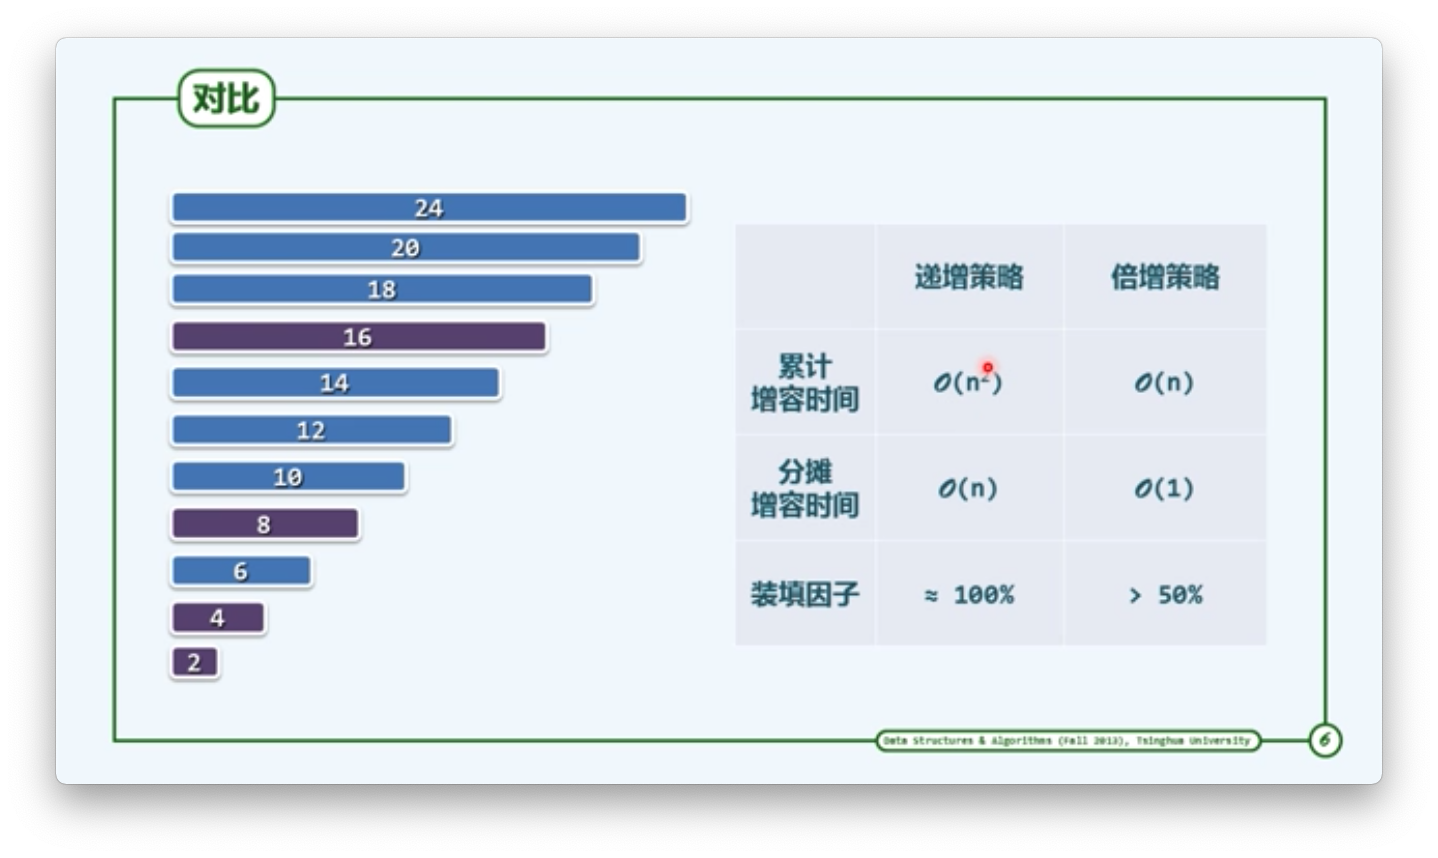
\includegraphics[scale=0.5]{3-2}

\subsection{分析方法}
\begin{itemize}
\item 平均分析
\item 分摊分析
\end{itemize}

\section{Binary Search}
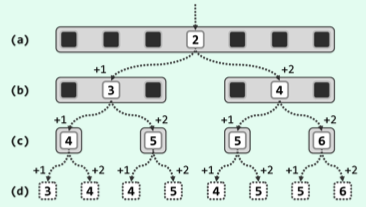
\includegraphics[scale=0.5]{3-3}

两次比较是因为有两次小于的比较,$e < s[mid]$,$s[mid] < e$, $O(1.5)lg n$

\section{Fibonacci Search}
\begin{itemize}
\item BS的左侧代价小,将左侧的长度设置更大,抵消右侧的开销
\item $O\left(1.44 \cdot \mathrm{lg}_{2} \mathrm{n}\right)$
\end{itemize}

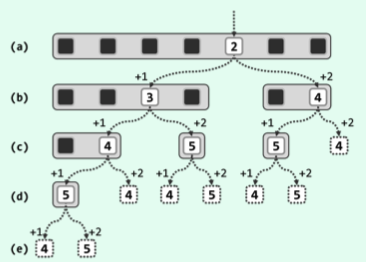
\includegraphics[scale=0.5]{3-4}

\section{二分查找B版}
\begin{itemize}
\item 三分支到两分支,mid 被归到右侧区间,不进行二次小于号比对,$O(\operatorname{logn})$
\end{itemize}
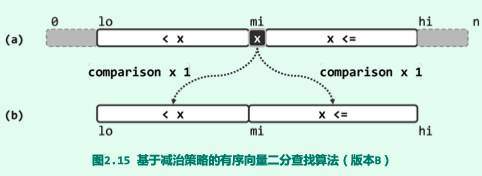
\includegraphics[scale=0.5]{3-5}

\section{二分查找C版}
\begin{itemize}
    \item $e < mid,\ hi = mi$
    \item $e \leq mid,\ hi = mi$
\end{itemize}

\section{排序及其分类}
\begin{itemize}
\item 内部排序
\begin{itemize}
\item 处理数据规模不大,可以在内存中处理
\end{itemize}
\item 外部排序
\begin{itemize}
\item 数据规模大,需要分布式存储器
\end{itemize}
\item offline Algorithms: 待排序数据批处理形式
\item online algorithms:待排序数据网络生成
\end{itemize}

\subsection{比较树(comparison tree)}
基于比较式算法(comparison-based algorithm),简称CBA式算法

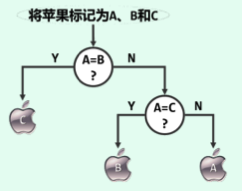
\includegraphics[scale=0.5]{3-6}

\subsection{bubble sort}
\paragraph{改进}
记录最后右侧反转的位置,缩小右侧的反转空间;反向排序记录最左侧的反转位置,缩小左侧的空间,从而不断地缩小需要排序的序列。

\section{mergesort}
\begin{itemize}
\item $O(\mathrm{nlogn})$
\item 两个有序向量合并一个有序向量:先sort再merge
\begin{itemize}
\item 递归可不断划分为子向量直到规模抵达递基
\item 递归返回的过程中不断归并
\end{itemize}
\end{itemize}
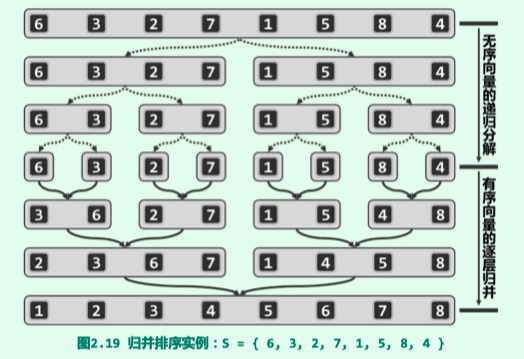
\includegraphics[scale=0.5]{3-7}

\subsection{改进}
判断条件的改进,对于前一个资源对比完成的对比组,后一个剩余的资源无需再更改,直接与原数组是对应的。

\section{Bitmap}
bitmap中存储的是bool值,其对应的


\chapter{列表}
\begin{itemize}
\item vector是 call-by-rank
\begin{itemize}
\item 对应逻辑和物理秩序
\item 读写操作容易,插入和移除操作难
\end{itemize}
\item 列表是call-by-position/call-by-link, 
\begin{itemize}
\item 因为放置的物理位置不连续,元素之间通过索引链接,仅仅对应逻辑秩序
\item 读写操作难,插入和移除操作容易
\end{itemize}
\end{itemize}

\section{insertionsort}
\begin{itemize}
\item 算法分为有序的前缀和无序的后缀
\item 反复将后缀元素转移至前缀
\end{itemize}

\section{selectionsort}
\begin{itemize}
\item 无序前缀,有序后缀
\item 后缀一直有序且不小于前缀
\end{itemize}

\section{mergesort}
\begin{itemize}
\item 复杂度$O(n \log n)$
\end{itemize}

\chapter{栈与队列}
\begin{itemize}
\item 线性列表
\item 操作仅限于逻辑上某端
\item 基本数据结构以硬件形式实现
\item 结构更为简化和紧凑,可以视作向量和列表的特例
\item eg: 网页浏览,文本编辑
\end{itemize}

\section{栈(stack)}
\begin{itemize}
\item last-in-first-out, LIFO
\end{itemize}

\subsection{栈与递归}
\begin{itemize}
\item 所需空间量取决于递归深度,最深的时候达到最多的递归实例
\item 递归调用和被调用函数实例关系存储在栈中
\begin{itemize}
\item 调用栈
\begin{itemize}
\item 跟踪统一程序的所有函数
\item 记录相互之间的调用关系
\item 执行完后保证准确返回
\item 基本单位是帧,每次函数调用创建一帧: 返回地址、传入参数、局部变量
\item 当期间发生新的调用会将新的调用压入栈顶,结束之后被中断的调用重新成为栈顶
\end{itemize}
\item 执行栈
\end{itemize}
\end{itemize}
\comment{尽量避免递归的使用,各种参数悉数入站难以统一优化,空间利用率非常低}

\section{栈的典型应用}
\begin{itemize}
\item 解以现行序列给出,序列逆序计算输出
\item 输入输出规模不确定
\end{itemize}

\subsection{逆序输出}
\subsection{递归嵌套}
括号匹配算法
\subsection{延迟缓冲}
\subsection{逆波兰表达式---RPN}

\section{试探回溯法}
\subsection{剪枝 pruning}
根据候选解的某些局部特征,以候选解子集为单位批量地排除。
\subsection{试探 probing}
从零开始,尝试 逐步增加候选解的长度。更准确地,这一过程是在成批地 考查具有特定前缀的所有候选解。从长度上逐步向目 标解靠近的尝试
\subsection{回溯 backtracking}
作为解的局部特 征,特征前缀在试探的过程中一旦被发现与目标解不合, 则收缩到此前一步的长度,然后继续试探下一可能的组合。

\section{队列 queue}
对象只能从一端进入(enqueue),另一端删除(dequeue),first-in-first-out, FIFO

\chapter{二叉树}
semi-linear structure 
\begin{itemize}
\item 连通无环图:顶点+边,有根(rooted tree)
\item depth,深度: 节点到根节点的边数
\item ancestor, descendant, proper ancestor(除自身外), proper descentdant
\item parent, child
\item degree(v的孩子总数), leaf(叶节点,无孩子的节点)
\item internal node(非root, leaf节点)
\item subtree
\item height(深度最大值)
\end{itemize}

\section{二叉树 binary tree}

\section{多叉树 k-ary tree}
每个节点的孩子均不超过$k$个的有根树

有序多叉树 = 二叉树\\
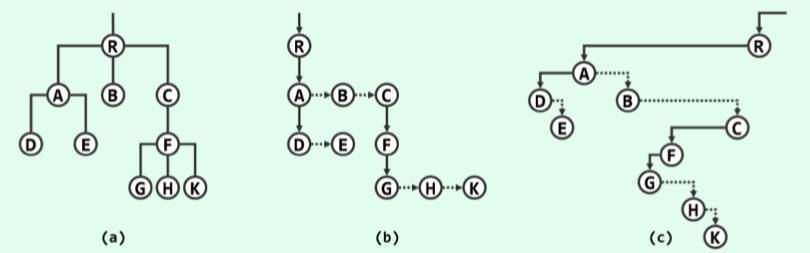
\includegraphics[scale=0.5]{5-1}

\section{编码树}
\subsection{二进制编码}
\begin{itemize}
\item 编码: 信息被转换为二进制形式
\item 解码: 二进制编码恢复原始信息
\item 前缀无歧义编码(prefix-free code), PFC编码
\end{itemize}
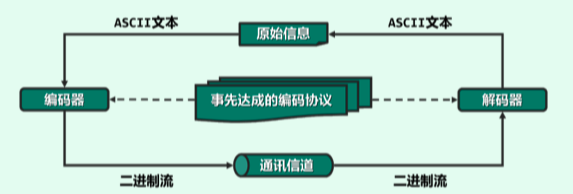
\includegraphics[scale=0.5]{5-2}


\subsection{二叉编码树}
PFC,所有的字符对应于叶子节点

\section{二叉树实现}
\subsection{遍历}
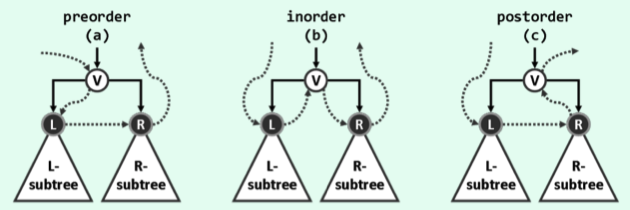
\includegraphics[scale=0.5]{5-3}

\subsection{迭代版先序遍历}
自顶而下访问左节点,每一个左节点都是当前节点的一部分,对应的右节点入栈,在自底而上访问右节点\\
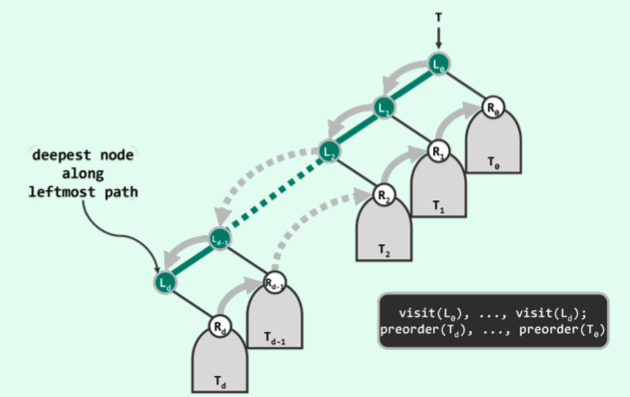
\includegraphics[scale=0.5]{5-4}

\subsection{迭代版中序遍历}
自顶而下沿着左节点深入,但是并不访问对应节点,而是直接入栈,直到无左孩子,再弹出入栈节点,访问该节点并转向右子树,重复左节点的方法,遍历完成右子树\\
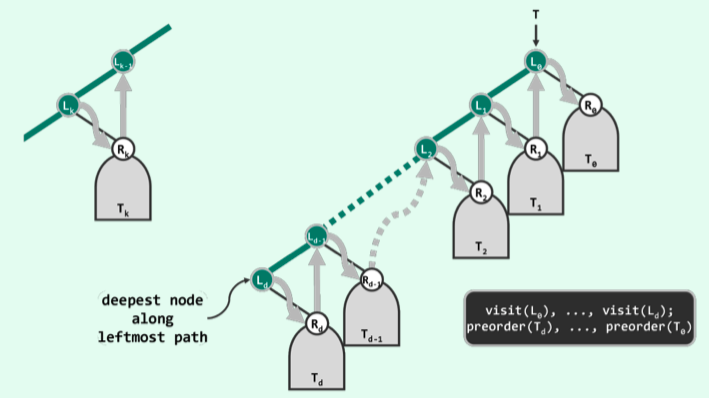
\includegraphics[scale=0.5]{5-5}

\comment{此方法的缺陷是,最坏的情况可能出现所有节点入栈,极大的空间消耗}

\subsection{改进迭代版中序遍历}
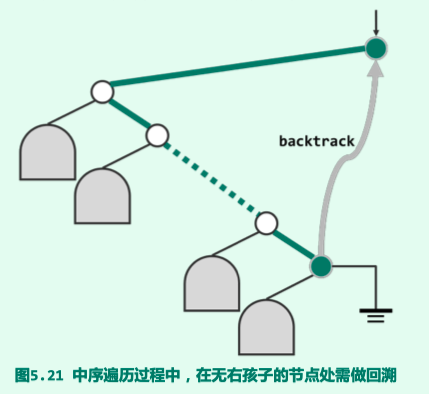
\includegraphics[scale=0.5]{5-6}\\
之前的节点都实施了入栈的行为,耗费空间,可以直接深入左节点直至最后一个,此时无左子树直接访问该节点,再判断有无右子树,如果有右子树,则需要重复之前的步骤进行遍历同时关闭回溯标志;如果右子树为空,则回溯同时设置回溯标志位为真,此时相当于直接访问回溯的

\subsection{迭代版后序遍历}
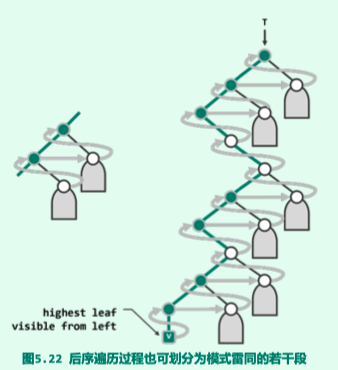
\includegraphics[scale=0.5]{5-7}\\
\begin{itemize}
\item ~\\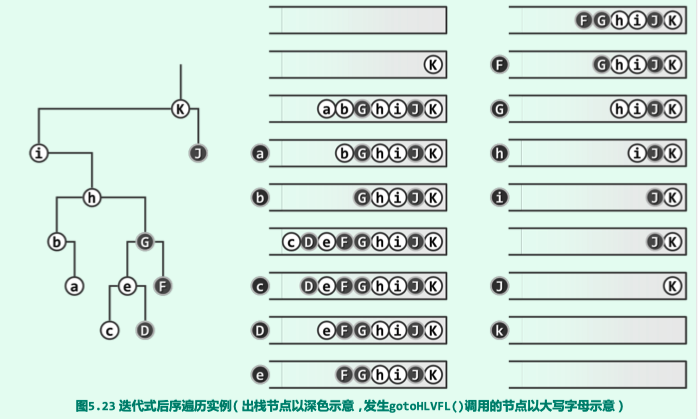
\includegraphics[scale=0.5]{5-8}
\item 入根节点(栈顶非根节点之父)
% \item 再入右侧子节点,再入左侧(重点,HLVFL节点)
\begin{itemize}
\item 左侧有子节点
\begin{itemize}
\item 右侧有子节点,先入右侧再入左侧
\item 右侧无子节点,直接入左侧
\end{itemize}
\item 左侧无,直接入右侧
\item 循环条件是不断赋值栈顶,只有当没有节点可深入才结束(最后结束是入左侧,那么左侧是重点,无左侧则右侧是重点)
\end{itemize}
\item 弹出终端节点进行访问,当栈顶又是非空右侧节点时,重复类似根节点的工作
\end{itemize}

\subsection{层次遍历}
广度优先遍历/层次遍历(level-order traversal):先上后下、先左后右
\\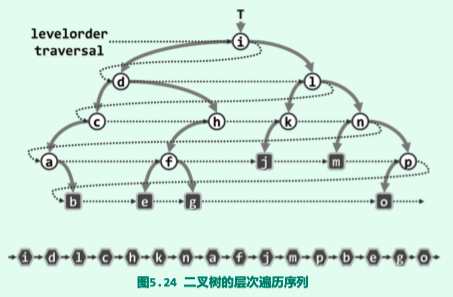
\includegraphics[scale=0.5]{5-9}
\begin{itemize}
\item 访问父节点
\item 子节点(左右)入队列,先访问左子节点,左子节点的子节点入队列,以此类推,直至到达底部返回
\end{itemize}

\paragraph{完全二叉树}
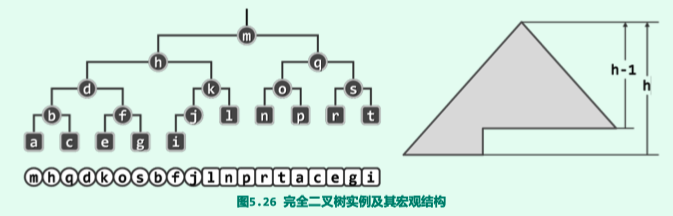
\includegraphics[scale=0.5]{5-11}\\
次底层之上所有父节点都有完全子节点,最底层叶节点都处于次底层叶节点的左侧,规模$2^h\sim 2^{h+1}-1$

\paragraph{满二叉树}
最底层的节点全满,完全二叉树的特例,有$2^{h+1}-1$个节点

\section{huffman 编码}
\subsection{PFC编码及解码}
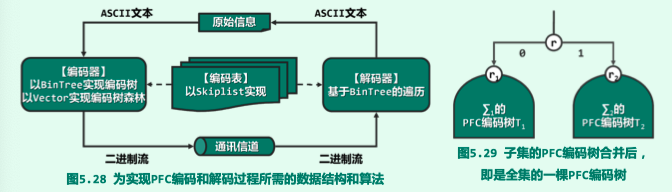
\includegraphics[scale=0.5]{5-12}\\

\subsection{最优编码树 optimal encoding tree}
$\operatorname{ald}(T)=\sum_{x \in \Sigma}|\operatorname{rps}(x)| /|\Sigma|=\sum_{x \in \Sigma} \operatorname{depth}(x) /|\Sigma|$

\begin{itemize}
\item {\bf 双子性}:真二叉树,左右孩子双全
\item {\bf 层次性}: 深度之差不得超过1  
\item 2|$\Sigma$| - 1的完全二叉树T,再 将中的字符任意分配给$T$的|$\Sigma$|个叶节点
\end{itemize}

\subsection{Huffman 编码树}
\begin{itemize}
\item 字符出现有概率
\item 带权平均编码长度与叶节点带权平均深度(weighted average leaf depth, WALD):$\operatorname{wald}(T)=\sum_{x \in \Sigma} p(x) \cdot|\operatorname{rps}(x)|$
\item 完全二叉树不能保证 WALD 最短
\item 最优带权编码树
\begin{itemize}
\item {\bf 双子性}:概率最低的是最底层的兄弟节点
\item {\bf 层次性}: 
\end{itemize}
\end{itemize}

\paragraph{算法}

对于$\Sigma$个已知字符,分别建立$\Sigma$棵树,每棵树对应的权重为该字符出现的频率,形成一个森林。从森林中取出权重最小的两棵树作为左、右子树,创建一个新的节点,权重为两棵子树的权重之和。反复迭代,每轮减少一棵树,最终形成一整棵高树,即huffman编码树。总体运行时间: $O(n)+o(n-1)+\ldots+o(2)=o\left(n^{2}\right)$

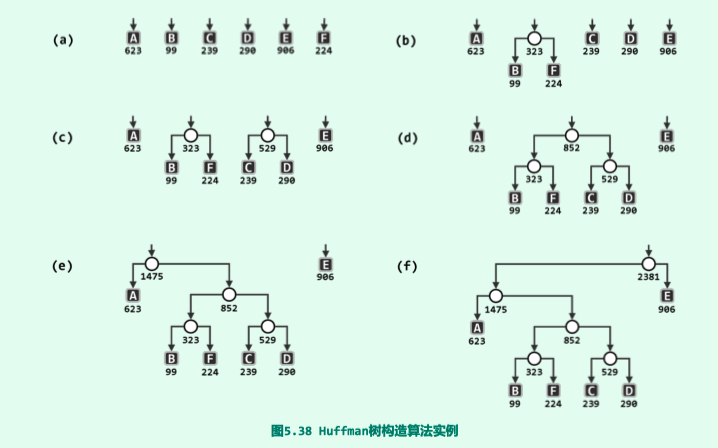
\includegraphics[scale=0.5]{5-14}

\chapter{图}
non-linear structure

\comment{通过遍历转化成semi-linear structure, 再通过树结构转化成线性结构}

\begin{itemize}
\item graph: $G=(V, E)$
\begin{itemize}
\item undirected graph/undigraph
\item directed graph/digraph
\item mixed graph
\item simple graph: 不含任何自环的图
\item directed acyclic graph, DAG
\item weighted graph/ network 
\end{itemize}
\item vertex: 顶点, 规模 $n=|V|$
\item edge: $E$, $e=|E|$
\begin{itemize}
\item undirected edge: $(u,v)$无次序
\item directed edge: $(u,v)$和$(v,u)$不对等
\end{itemize}
\item degree: 与顶点相连的边数
\begin{itemize}
\item in-degree: incoming edge
\item out-degree: outgoing edge
\end{itemize}
\item simple path: 沿途顶点互异
\item Eulerian tour: 欧拉环路, 经过途中各边一次且恰好一次的环路
\end{itemize}

\section{邻接矩阵 adjacency matrix}
\begin{itemize}
\item 访问时间$O(1)$
\item 顶点动态操作接口耗时
\item 空间冗余大,vector装填因子不低于50\%, 单次操作耗时不过$O(n^2)$
\end{itemize}

\section{邻接表 adjacency list}
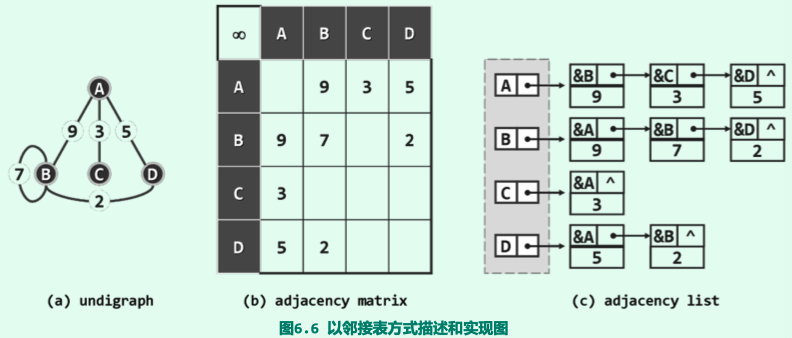
\includegraphics[scale=0.5]{5-15}
\begin{itemize}
\item 空间总量$O(n+e)$
\item 时间复杂度,反问单条边的效率不高,但是擅长批量处理方式
\item 总体效率比邻接矩阵要高
\end{itemize}

\section{图算法}
graph search: 对处于特定状态顶点的甄别与查找
\subsection{广度优先搜索 breath-first search, BFS}
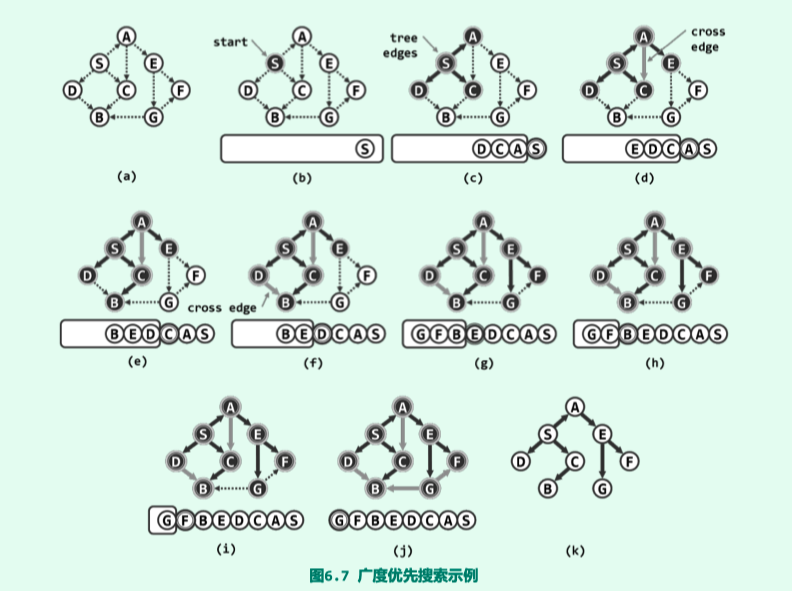
\includegraphics[scale=0.5]{5-16}
\begin{itemize}
\item 层次遍历
\item frontier,前沿集中的所有顶点的深度相差不超过1
\item 覆盖无向图s所属的连通分量
\item 覆盖有向图s为起点的可达分量
\item 总体时间复杂度$O(n+e)$
\end{itemize}

\subsection{深度优先搜索 depth-first search, DFS}
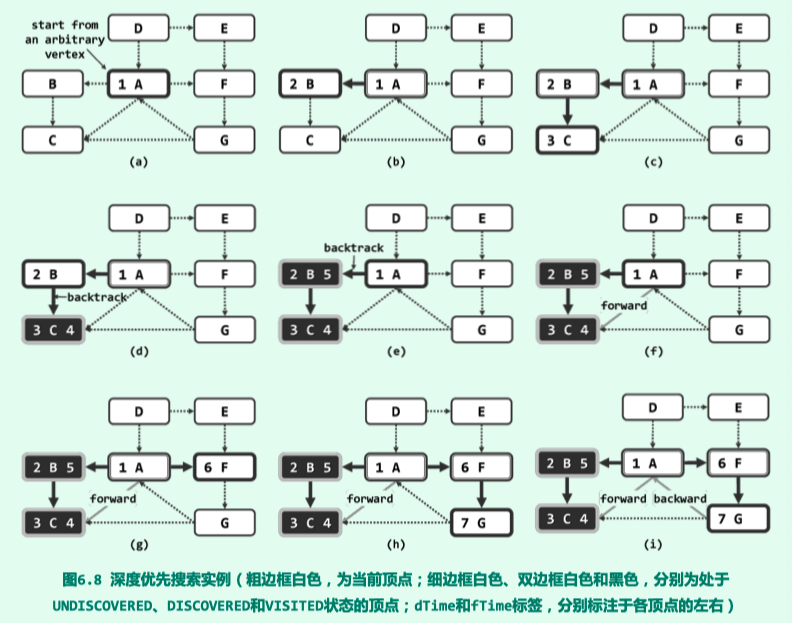
\includegraphics[scale=0.5]{5-17}\\
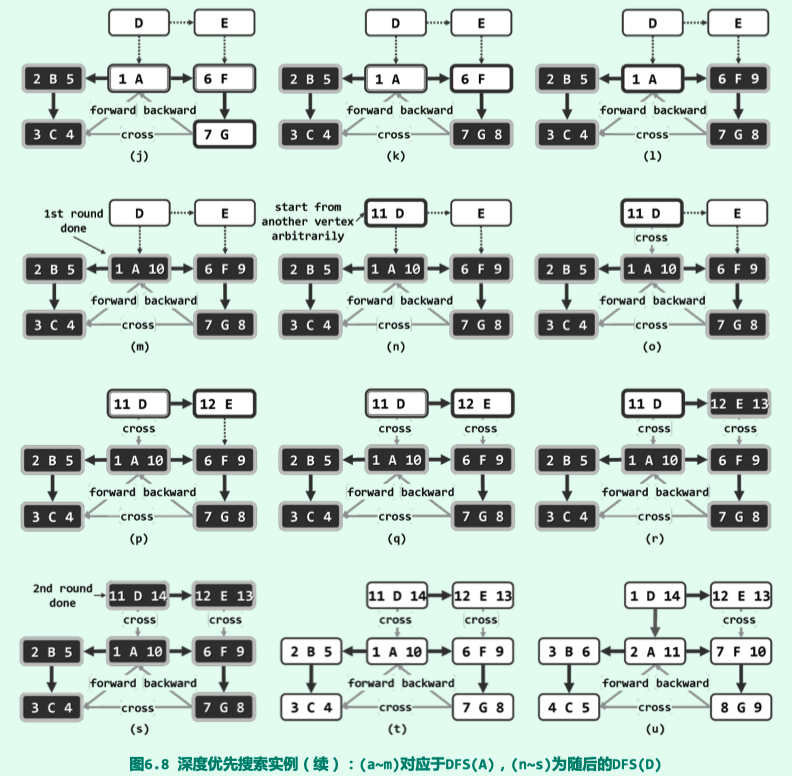
\includegraphics[scale=0.5]{5-18}\\

有两棵DFS树,起点不同,形成的DFS树也会不同\\
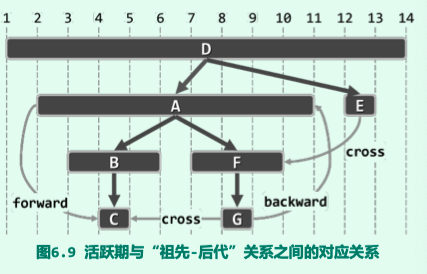
\includegraphics[scale=0.5]{5-19}
\begin{itemize}
\item 时间复杂度$O(n+e)$
\item 空间复杂度,需要耗费一定量空间
\end{itemize}

\section{拓扑排序 topological sorting}
每一顶点都不会通过边,指向其在此序列中的前驱顶点。

\subsection{有向无环图}
\begin{itemize}
\item 必然有拓扑排序
\item 必有入度为0的顶点(起点),极大顶点
\item 必有出度为0的顶点(终点),极小顶点
\end{itemize}

\section{双连通域分解}
\begin{itemize}
\item 切割节点/关节点: 删除顶点v后G所包含的连通域增多
\item 双连通图: 不含关节点的图
\end{itemize}
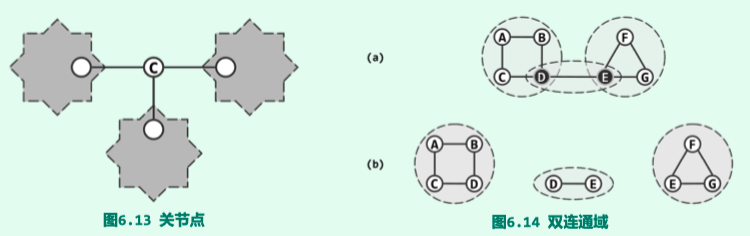
\includegraphics[scale=0.5]{5-20}

\subsection{蛮力算法}
\begin{itemize}
\item BFS或者DFS找到连通域的数目
\item 枚举删除顶点v,重新计算连通域
\item 连通域变化则是关节点,否则不是
\end{itemize}

\subsection{可行算法}
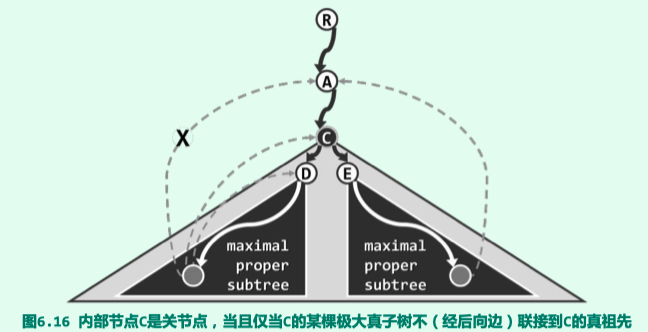
\includegraphics[scale=0.5]{5-21}
\begin{itemize}
\item 无向图DFS树中,在搜索过程中,更新各顶点所能连同的最高祖先(highest connected ancestor, HCA),即可认定关节点
\item $hca[{u}] \geq {dTime}[\mathrm{v}]$, 说明u及其后代无法通过后向边与v的真祖先连同,故v为关节点。
\item $hca[{u}] < {dTime}[\mathrm{v}]$, 说明u及其后代可通过后向边与v的真祖先连同,故v不为关节点。 
\end{itemize}

\section{优先级搜索}
priority-first search, PFS/ best-first search, BFS

以迭代的方式逐步引入顶点和边,最终构造出一颗遍历树,每次都引入当前优先级最高的顶点s,按照不同的策略更新其邻接顶点的优先级数。

\section{最小支撑树}
连通图G中的某一无环连通子图T若覆盖G中所有的顶点,则称为G的一棵支撑树或生成树(spanning tree)\\
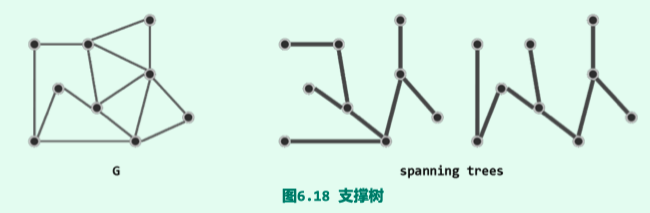
\includegraphics[scale=0.5]{5-22}
 
所有spinning tree中,成本最低者(边权重之和)为最小支撑树(minimum spanning tree, MST),不一定唯一

\subsection{蛮力算法}
由n个互异顶点组成的完全图共有$n^{n-2}$ 棵支撑树,更新成本记录需要$O(n^{n-2})$

\subsection{Prim 算法}
图 G=(V; E),顶点集V的任一非平凡自己U及其补集V\backslash U,构成图G的一个割cut, 其中两个子集之间相连接的边为crossing edge(跨越边/桥)。

\paragraph{贪心迭代}
阴影中的子图内的顶点始终至少与集合内至少一点相连,其余过大的边就删除掉,逐步扩充子图的顶点个数,不停迭代。

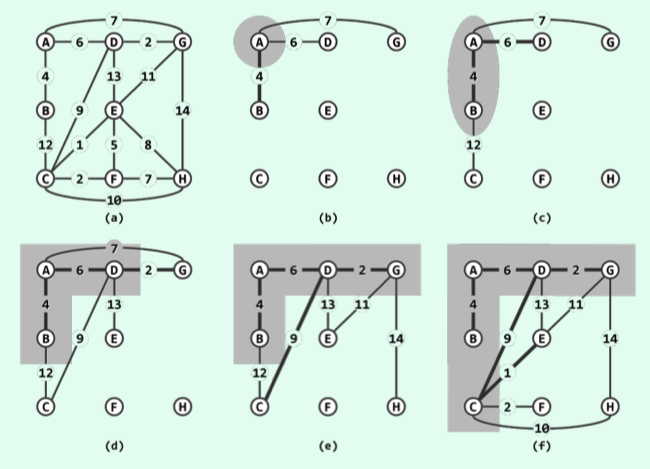
\includegraphics[scale=0.5]{5-23}\\
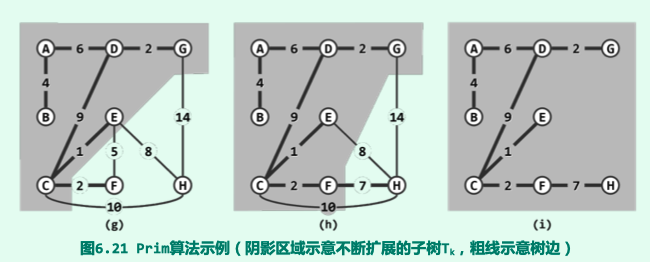
\includegraphics[scale=0.5]{5-24}

\section{最短路径}
最短路径的任一前缀也是最短路径

\subsection{Dijkstra算法}
与prim相比,Dijkstra算法关注的是每一个顶点到$s$距离最近者,而前者关注的是到$T_k$这个整体的最近者。

\chapter{搜索树}
\section{二叉搜索树}
\subsection{循关键码查询 call-by-key}
\paragraph{查找算法及其实现}
时间复杂度:$O(n)$最坏(当数字是顺序排列,就成了列表形式,查找最大值就是在最长的部分进行搜索)

\paragraph{插入算法}
在search算法的基础上进行,插入之后需要更新对应的祖先的高度,时间复杂度取决于search()和updateHeightAbove()的

\paragraph{删除算法}
单分支,直接替换即可;双分支需要找到合适的节点

\section{平衡二叉搜索树}
\subsection{随机生成 vs 随机组成}
\begin{itemize}
\item \stress{随机生成:}将$n$个值进行随机排列,因为顺序一般都会被打乱,那么最终生成的二叉树的深度不太可能是最坏的情况,平均高度是$\Theta(\log n)$
\item \stress{随机组成:}遵循一定顺序性的前提下,随机确定他们之间的拓扑连接,平均查找长度为 $\Theta(\sqrt{\mathrm{n}})$
\item 随机生成的高度不同于随机组成的高度,是因为随机生成的序列有很多序列不同、结构一样的二叉树被重复统计
\end{itemize}

\subsection{理想平衡 vs 适度平衡}
\begin{itemize}
\item \stress{理想平衡}:高度恰好为$\left\lfloor\log _{2} n\right\rfloor$
\item \stress{适度平衡}:树高渐进地不超过$O(\log n)$
\end{itemize}

\subsection{等价交换}
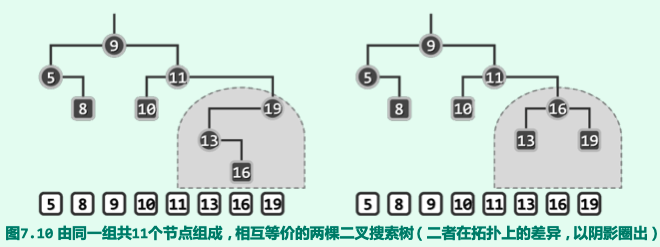
\includegraphics[scale=0.5]{5-25}
\paragraph{调整手段}
\begin{itemize}
\item zig
\item zag\\
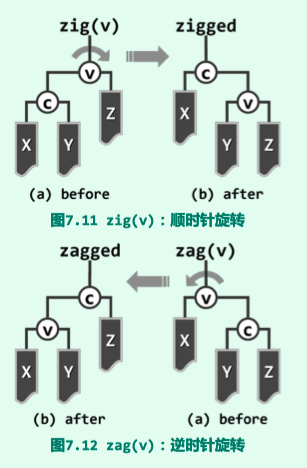
\includegraphics[scale=0.5]{5-26}
\end{itemize}

\section{AVL树}
\begin{itemize}
\item \stress{平衡因子}: balFac(v) = height(lc(v)) - height(rc(v))
\item \stress{失衡}:因节点的插入或删除而暂时失衡的节点构成失衡节点集,$UT(x)$
\item \stress{重失衡}:\\
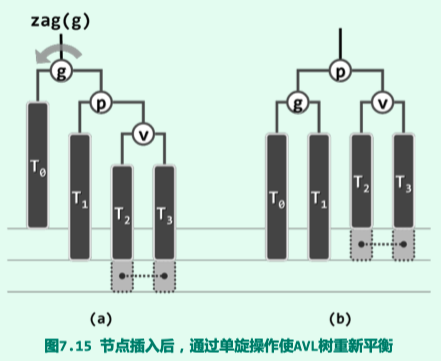
\includegraphics[scale=0.5]{5-27}\\
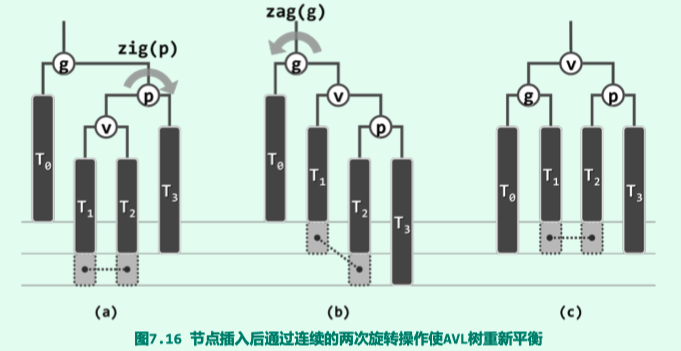
\includegraphics[scale=0.5]{5-28}
\end{itemize}

\subsection{统一重平衡算法}
上诉的重构涉及的较为复杂,可以根据``3+4''进行重构,失衡节点和对应的子树直接重新组装而不是旋转

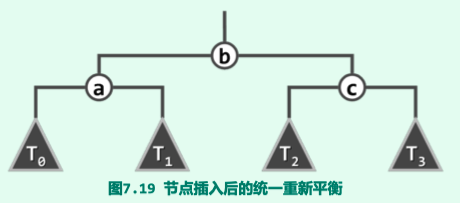
\includegraphics[scale=0.5]{5-29}

\chapter{高级搜索树}
\section{伸展树 splay tree}
\begin{itemize}
\item 数据局部性(data locality)
\begin{itemize}
\item 刚被访问的元素,可能不久之后再次被访问到
\item 将被访问的下一元素,可能处于不久之前就被访问过的某个元素的附近
\end{itemize}
\end{itemize}
\subsection{逐层伸展}
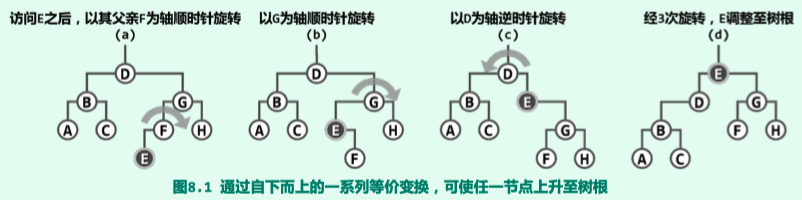
\includegraphics[scale=0.5]{5-30}
\begin{itemize}
\item 平均访问时间$\Omega\left(n\right)$
\end{itemize}

\subsection{双层伸展}
\begin{itemize}
\item zig-zig/zag-zag\\
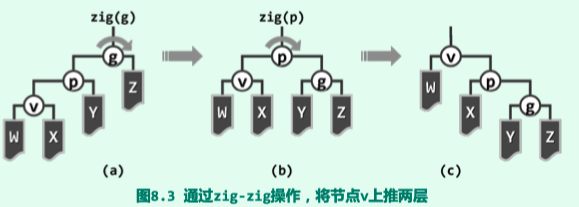
\includegraphics[scale=0.5]{5-32}
\item zig-zag/zag-zig\\
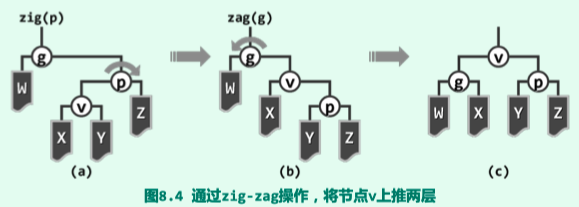
\includegraphics[scale=0.5]{5-33}
\item 双层伸展和单旋相结合可以完成节点的移动
\item 时间复杂度$O(\log n)$
\end{itemize}

\section{B-树}
\subsection{分级存储}
\begin{itemize}
\item 内存高速度
\item 外存大容量
\item 内、外之间的数据传输:I/O操作
\end{itemize}

\subsection{四路搜索树}
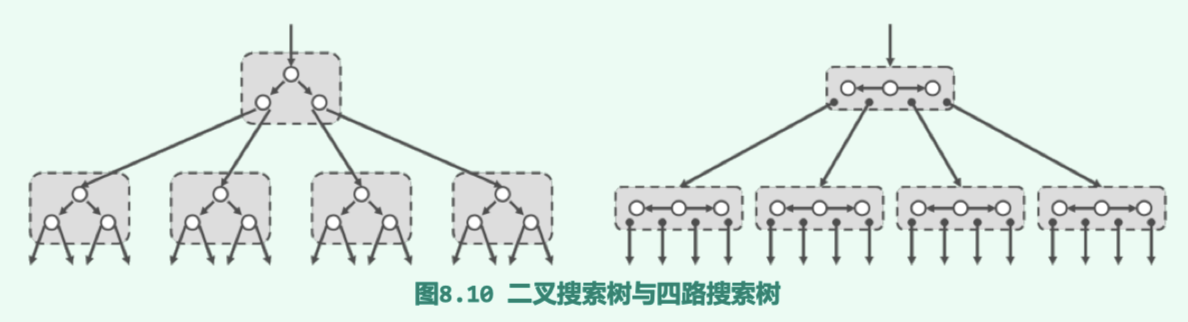
\includegraphics[scale=0.5]{5-34}
\begin{itemize}
\item 将二叉树中的两层转化为四路``大节点''
\item k层为间隔进行重组,可将二叉搜索树转化为$2^k$路搜索树,多路搜索树 multi-way search tree
\end{itemize}

\subsection{多路平衡搜索树}
m阶B-树(B-tree)

\paragraph{关键码查找}
\begin{itemize}
\item B-树适宜在相对更小的内存中,实现对大规模数据的高效操作
\item 
\end{itemize}

\paragraph{上溢与分裂}
\begin{itemize}
\item 关键码的删除会引发节点的上溢
\item 上溢节点提升为父节点,如果发生上溢上传,就一直传递,当传至根节点是,可以自成一个新的树根
\end{itemize}

\paragraph{下溢和合并}
关键码的插入会引发节点的下溢

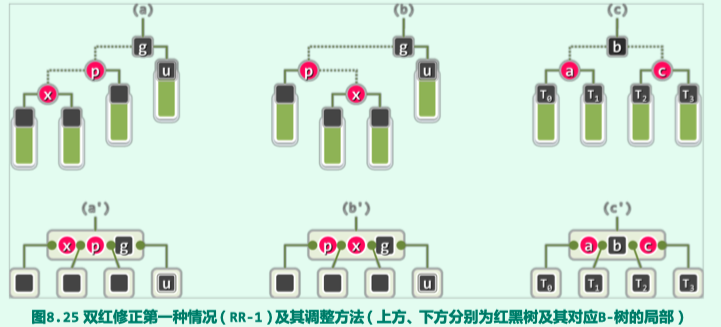
\includegraphics[scale=0.5]{5-37}\\
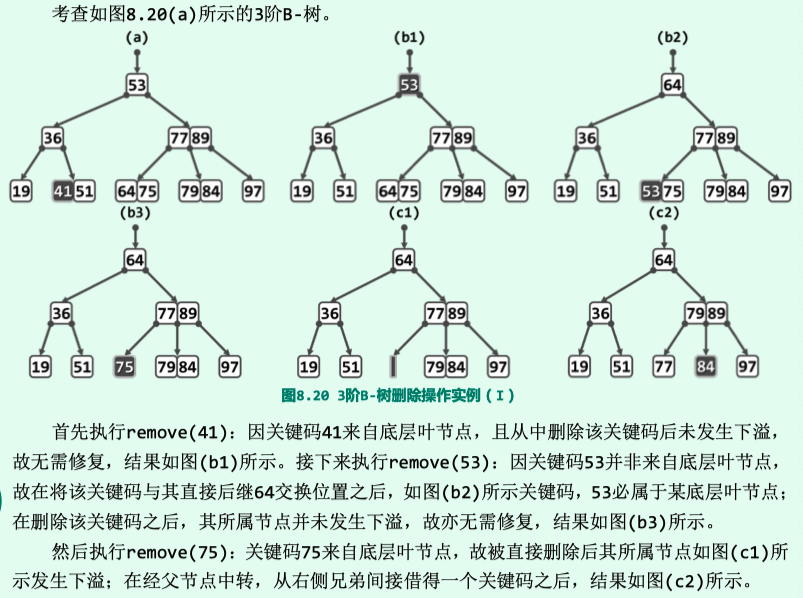
\includegraphics[scale=0.5]{5-38}


\section{红黑树}
\begin{itemize}
\item 树根始终为黑色
\item 外部节点均为黑色
\item 其余节点若为红色,则其孩子节点必为黑色
\item 从任一外部节点到根节点的沿途,黑节点的数目相等
\end{itemize}

\paragraph{红黑树到4阶B树的等效转换}
\begin{itemize}
\item 节点中黑码仅包含1个
\end{itemize}
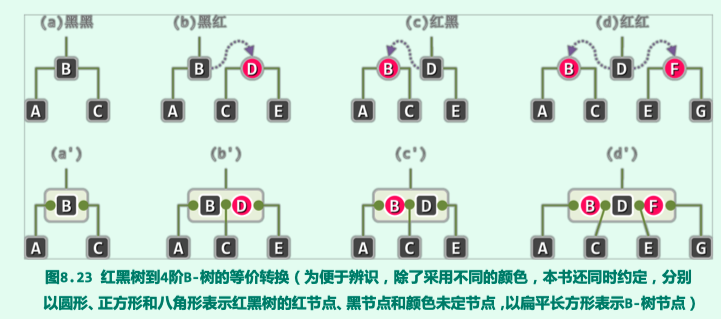
\includegraphics[scale=0.5]{5-35}

\paragraph{平衡性}
因为红黑树中任一通路都不包含相邻的红节点,那么搜索树的高度不会超过黑高度的两倍,虽然无法做到理想平衡,到那会其高度依然可控制在$O(\log n)$。此中的树高指的实际是红黑树的黑高度

\paragraph{查找算法}
查找节点,如果目标节点不存在,则在查找终止的位置创建节点,并随即将其染成红色(除非全树仅此一个节点才染黑)

\paragraph{插入算法}
引入红节点之后,可能出现双红现象
\begin{itemize}
\item 双红修正RR-1(另外有两种对称情况),u为黑色,出现双红的时候,x的孩子兄弟和u的黑高度均相等,需要修正\\
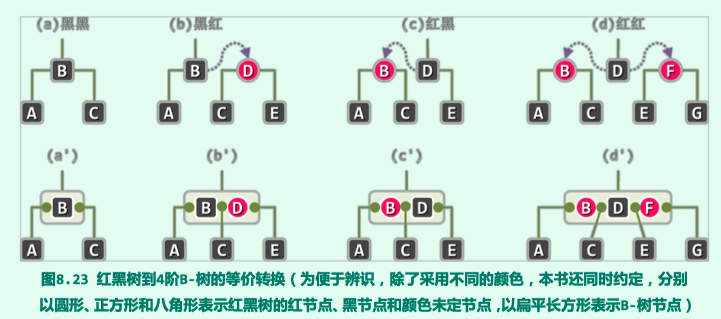
\includegraphics[scale=0.5]{5-36}
\item 双红修正RR-1(另外有两种对称情况), u为红色, 违反条件 (3)\\
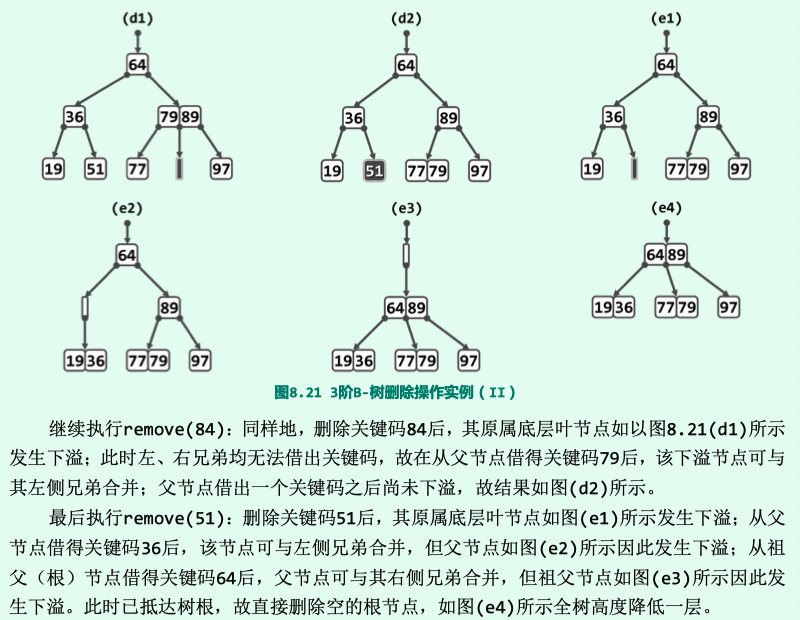
\includegraphics[scale=0.5]{5-39}
\end{itemize}
修正的复杂度:

% 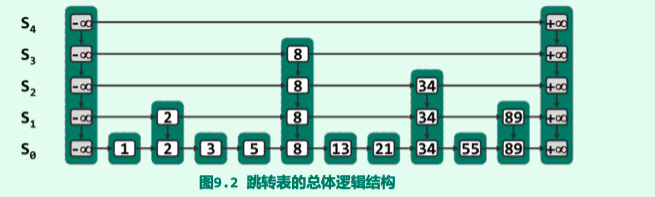
\includegraphics[scale=0.5]{5-42}

\paragraph{节点删除算法}
\begin{itemize}
\item 。。。
\end{itemize}



\section{kd-树}
\subsection{范围搜索}
\begin{itemize}
\item 1D:平衡二叉树
\item 2D~多维: 递归定义的平衡二叉搜索树 --- kd树
\end{itemize}








